\documentclass{article}
    \usepackage{amssymb}
    \usepackage[utf8]{inputenc}
    \usepackage[russian]{babel}
    \usepackage[left=2cm,right=2cm,
        top=2cm,bottom=2cm,bindingoffset=0cm]{geometry}
    \usepackage{hyperref}
    \hypersetup{
        colorlinks=true,
        linkcolor=blue,
        filecolor=magenta,      
        urlcolor=cyan,
    }
  \usepackage{graphicx}
  \graphicspath{{pictures/}}
  \DeclareGraphicsExtensions{.pdf,.png,.jpg}
\usepackage{subcaption}
%\captionsetup{compatibility=false}

\begin{document}
\begin{center}{\hugeОтчет по курсовой работе за неделю\\}\end{center}
Дата: 10.12.2020\\
Научные руководители: Герасимов С.В., Мещеряков А.В.\\
Студент: Немешаева Алиса\\
Курс: 4\\

\renewcommand{\labelitemi}{$\blacksquare$}
\renewcommand\labelitemii{$\square$}
\begin{enumerate}
    \item На этой неделе основная работа велась по дополнению материалов для 
        \href{https://www.overleaf.com/read/zcgvtyscsyhv}{статьи}.\\
    \item Также был написан текст выпускной работы на основе этой статьи.\\
    \item Были построены каталоги для моделей pz и pz\_act на эпохах 20 и 25, было проведено 
        сравнение.\\

        \begin{figure}[h]
            \center{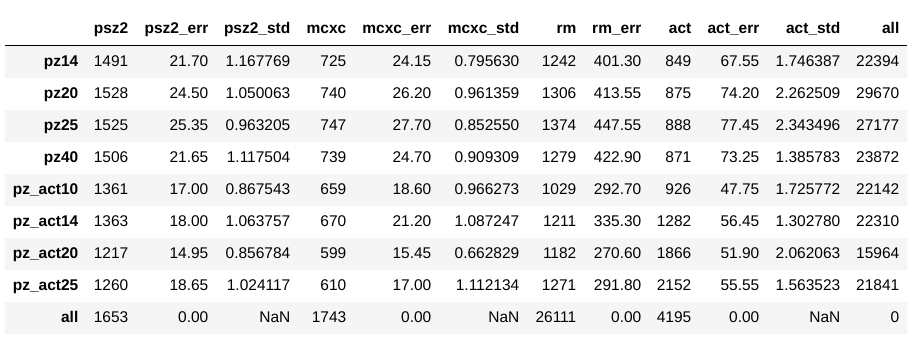
\includegraphics[width=0.7\linewidth]{comp}}
            \caption{Сравнение количества найденных объектов в разных каталогах}
        \end{figure}
\end{enumerate}

Отчет согласован с научным руководителем.\\
Общее количество строк кода за эту неделю: 178\\
\href{https://github.com/rt2122/data-segmentation-2}{Репозиторий}\\ 
\end{document}
